% This is text associated with the open textbook "Open Electromagnetics"
% See immediately below for author, date
% This work is licensed under the Creative Commons Attribution-ShareAlike 4.0 International License. (CC BY-SA 4.0) 
% To view a copy of the license, visit http://creativecommons.org/licenses/by-sa/

%ORB TITLE Induction in a Motionless Loop
%ORB AUTHOR 0        # S.W. Ellingson, Virginia Tech (ellingson@vt.edu)
%ORB DATE 20180807   # yyyymmdd
%ORB ABSTRACT Current Induced in a Motionless Planar Loop by a Spatially-Uniform Time-Varying Magnetic Field

% original (long) title: "Induction in a Motionless Loop by a Spatially-Uniform Time-Varying Magnetic Field"

\label{m0056_Current_Generated_by_a_Single_Loop_in_a_Time-Varying_Magnetic_Field} % <-- Must match name of this file and module directory name.  Don't mess with this!
\index{emf!transformer|(}

In this section, we consider the problem depicted in Figure~\ref{m0056_fPS}, which is a single motionless loop of wire in the presence of a spatially-uniform but time-varying magnetic field.  A small gap is introduced in the loop, allowing us to measure the induced potential $V_T$.  Additionally, a resistance $R$ is connected across $V_T$ in order to allow a current to flow.
This problem was considered in Section~\ref{m0055_Faradays_Law} as an introduction to Faraday's Law; in this section, we shall actually work the problem and calculate some values.
This is intended to serve as an example of the application of Faraday's Law, a demonstration of transformer emf, and will serve as a first step toward an understanding of transformers as devices.
%
\begin{figure}[b!]
\begin{center}
\pdftooltip{{  % note double braces
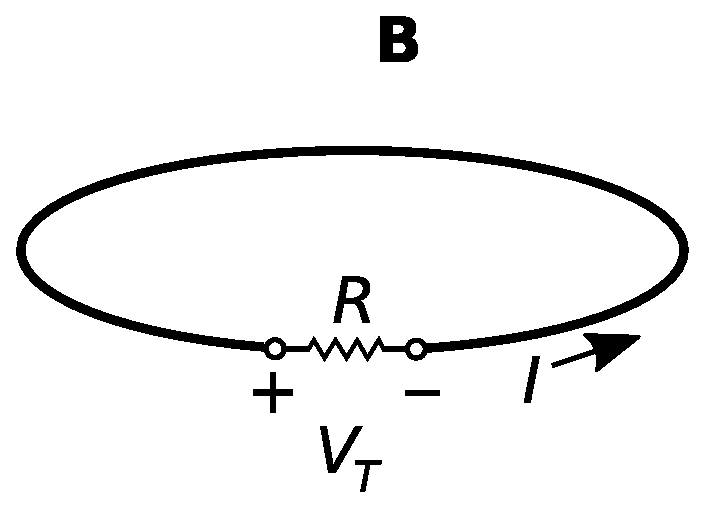
\includegraphics[width=2.5in]{modules/m0055_fFaradaySingleLoop.eps}
% ***WikipediaCommonsURL
}}{A loop of wire lying in a magnetic field, B. In the loop lies a resistor, R, between a positive and negative node. Beneath the resistor is labeled V sub T. A vector, I, on the right points in a counterclockwise direction.}
\end{center} 
%\centerline{\scriptsize 
%\copyright~\hyperref[***_Credit]{author} 
%\href{https://creativecommons.org/licenses/by-sa/4.0/}{CC BY-SA 4.0} 
%} 
\caption{
\label{m0056_fPS}
A single loop of wire in the presence of an impressed spatially-uniform but time-varying magnetic field.
}
\end{figure}

In the present problem, the loop is centered in the $z=0$ plane.
The magnetic flux density is ${\bf B} = \hat{\bf b}B(t)$; i.e., time-varying magnitude $B(t)$ and a constant direction $\hat{\bf b}$.
Because this magnetic field is spatially uniform (i.e., the same everywhere), we will find that only the area of the loop is important, and not it's specific shape.
For this reason, it will not be necessary to specify the radius of the loop or even require that it be a circular loop. 
Our task is to find expressions for $V_T$ and $I$.

To begin, remember that Faraday's Law is a calculation of electric potential and not current.
So, the approach is to first find $V_T$, and then find the current $I$ that flows through the gap resistance in response.
  
The sign convention for $V_T$ is arbitrary; here, we have selected ``$+$'' and ``$-$'' terminals as indicated in Figure~\ref{m0056_fPS}.\footnote{A good exercise for the student is to repeat this problem with the terminal polarity reversed; one should obtain the same answer.}
Following the standard convention for the reference direction of current through a passive device, $I$ should be directed as shown in Figure~\ref{m0056_fPS}.
It is worth repeating that these conventions for the signs of $V_T$ and $I$ are merely \emph{references}; for example, we may well find that $I$ is negative, which means that current flows in a clockwise direction in the loop. 

We now invoke Faraday's Law:
\index{Faraday's law}
%
\begin{equation}   
V_T = - N \frac{\partial}{\partial t} \Phi 
\end{equation}
%
The number of windings $N$ in the loop is 1, and $\Phi$ is the magnetic flux through the loop.  Thus:
%
\begin{equation}   
V_T = - \frac{\partial}{\partial t} \int_{\mathcal{S}} { {\bf B} \cdot d{\bf s} }
\end{equation}
%
where $\mathcal{S}$ is any open surface that intersects all of the magnetic field lines that pass through the loop.
The simplest such surface is simply the planar surface defined by the perimeter of the loop.
Then $d{\bf s}=\hat{\bf n}ds$, where $ds$ is the differential surface element and $\hat{\bf n}$ is the normal to the plane of the loop.
Which of the two possible normals to the loop?
This is determined by the right-hand rule 
\index{right-hand rule!Stokes' theorem}
of Stokes' Theorem.
\index{Stokes' theorem}
From the ``$-$'' terminal, we point the thumb of the right hand in the direction that leads to the ``$+$'' terminal by traversing the perimeter of the loop.
When we do this, the curled fingers of the right hand intersect $\mathcal{S}$ in the same direction as $\hat{\bf n}$.
To maintain the generality of results derived below, we shall not make the substitution $\hat{\bf n}=+\hat{\bf z}$; nevertheless we see this is the case for a loop parallel to the $z=0$ plane with the polarity of $V_T$ indicated in Figure~\ref{m0056_fPS}.

Taking this all into account, we have
%
\begin{flalign}   
V_T &= - \frac{\partial}{\partial t} \int_{\mathcal{S}} { \left(\hat{\bf b}B(t)\right) \cdot \left(\hat{\bf n}ds\right) } \nonumber \\
    &= - \left(\hat{\bf b}\cdot\hat{\bf n}\right) \frac{\partial}{\partial t} \int_{\mathcal{S}} {B(t)~ds } 
\end{flalign}
%
Since the magnetic field is uniform, $B(t)$ may be extracted from the integral.
Furthermore, the shape and the orientation of the loop are time-invariant, so the remaining integral may be extracted from the time derivative operation.
This leaves:
%
\begin{flalign}   
V_T = - \left(\hat{\bf b}\cdot\hat{\bf n}\right) \left( \frac{\partial}{\partial t} B(t) \right)  \int_{\mathcal{S}} { ds } 
\end{flalign}
%
The integral in this expression is simply the area of the loop, which is a constant; let the symbol $A$ represent this area.
We obtain
%
\begin{equation}  
\boxed{ 
V_T =  - \left(\hat{\bf b}\cdot\hat{\bf n}A\right) \frac{\partial}{\partial t} B(t)
}
\label{m0056_eVT}
\end{equation}
% 
which is the expression we seek.
Note that the quantity $\hat{\bf b}\cdot\hat{\bf n}A$ is the \emph{projected area} of the loop.
The projected area is equal to $A$ when the the magnetic field lines are perpendicular to the loop (i.e., $\hat{\bf b}=\hat{\bf n}$), and decreases to zero as $\hat{\bf b}\cdot\hat{\bf n}\to 0$.
Summarizing:
%
%ORB HIGHLIGHT
\begin{mdframed}[backgroundcolor=yellow!20,nobreak=true] 
The magnitude of the transformer emf induced by a spatially-uniform magnetic field is equal to the projected area times the time rate of change of the magnetic flux density, with a change of sign. (Equation~\ref{m0056_eVT}).
\end{mdframed}

A few observations about this result:  
%
\begin{itemize}
\item As promised earlier, we have found that the shape of the loop is irrelevant; i.e., a \emph{square} loop having the same area and planar orientation would result in the same $V_T$.  This is because the magnetic field is spatially uniform, and because it is the magnetic flux ($\Phi$) and not the magnetic field or shape of the loop alone that determines the induced potential. 
\item The induced potential is proportional to $A$; i.e., $V_T$ can be increased by increasing the area of the loop. 
\item The peak magnitude of the induced potential is maximized when the plane of the loop is perpendicular to the magnetic field lines.  
\item The induced potential goes to zero when the plane of the loop is parallel to the magnetic field lines.  Said another way, there is no induction unless magnetic field lines pass through the loop.   
\item The induced potential is proportional to the rate of change of ${\bf B}$.  If ${\bf B}$ is constant in time, then there is no induction.
\end{itemize}

Finally, the current in the loop is simply
%
\begin{equation}
I = \frac{V_T}{R}
\end{equation}
%
Again, electromagnetic induction induces potential, and the current flows only in response to the induced potential as determined by Ohm's Law.
In particular, if the resistor is removed, then $R\to\infty$ and $I\to0$, but $V_T$ is unchanged.

One final comment is that even though the current $I$ is not a \emph{direct} result of electromagnetic induction, we can use $I$ as a check of the result using Lenz's Law
\index{Lenz's law}
(Section~\ref{m0129_Electromagnetic_Induction}).  We'll demonstrate this in the example below.

%%%%%%%%%%%%%%%%%%%%%%%%%%%%%%%%%%%%%%%%%%%%%%%
%ORB EXAMPLE
~\\ \begin{example} 
\begin{mdframed}[backgroundcolor=brown!20,linecolor=brown!20]\raggedright
Induction in a motionless circular loop by a \emph{linearly}-increasing magnetic field
\\~\\
Let the loop be planar in the $z=0$ plane and circular with radius $a=10$~cm.
Let the magnetic field be $\hat{\bf z}B(t)$ where
%
\begin{flalign}
B(t) &=0       ~~~~~~~~\mbox{,}~t<0 \nonumber \\
     &=B_0 t/t_0 ~\mbox{,}~0\le t \le t_0 \nonumber \\
     &=B_0     ~~~~~~\mbox{,}~t>t_0 
\end{flalign}
%
i.e., $B(t)$ begins at zero and increases linearly to $B_0$ at time $t_0$, after which it remains constant at $B_0$.
Let $B_0=0.2$~T, $t_0=3$~s, and let the loop be closed by a resistor $R=1~\mbox{k}\Omega$.
What current $I$ flows in the loop? 

{\bf Solution}.   
Adopting the sign conventions of Figure~\ref{m0056_fPS} we first note that $\hat{\bf n}=+\hat{\bf z}$; this is determined by the right-hand rule with respect to the indicated polarity of $V_T$.
Thus, Equation~\ref{m0056_eVT} becomes
%
\begin{equation}  
V_T =  - \left(\hat{\bf b}\cdot\hat{\bf z}A\right) \frac{\partial}{\partial t} B(t)
\nonumber
\end{equation}
%
Note $\hat{\bf b}\cdot\hat{\bf z}A=A$ since $\hat{\bf b}=\hat{\bf z}$; i.e., because the plane of the loop is perpendicular to the magnetic field lines.
Since the loop is circular, $A = \pi a^2$. 
Also
%
\begin{flalign}
\frac{\partial}{\partial t}B(t) &=0       ~~~~~~~~\mbox{,}~t<0 \nonumber \\
                 &=B_0/t_0 ~\mbox{,}~0\le t \le t_0 \nonumber \\
                 &=0     ~~~~~~~\mbox{,}~t>t_0 \nonumber
\end{flalign}
%
Putting this all together:
%
\begin{equation}  
V_T =  -\pi a^2 \frac{B_0}{t_0} = -2.09~\mbox{mV} ~\mbox{,}~0\le t \le t_0
\nonumber
\end{equation}
%
and $V_T=0$ before and after this time interval, since ${\bf B}$ is constant during those times.
Subsequently the induced current is
%
\begin{equation}   
I = \frac{V_T}{R} = -2.09~\mu\mbox{A} ~\mbox{,}~0\le t \le t_0
\nonumber
\end{equation}
%
and $I=0$ before and after this time interval.
We have found that the induced current is a constant clockwise flow that exists only while ${\bf B}$ is increasing. 

Finally, let's see if the result is consistent with Lenz's Law.
\index{Lenz's law}
The current induced while ${\bf B}$ is changing gives rise to an induced magnetic field ${\bf B}_{ind}$.   
From the right-hand rule 
\index{right-hand rule!magnetic field of a wire}
that relates the direction of $I$  to the direction of ${\bf B}_{ind}$ (Section~\ref{m0119_Magnetic_Field_of_a_Long_Wire}), the direction of ${\bf B}_{ind}$ is generally $-\hat{\bf z}$ inside the loop.  
In other words, the magnetic field associated with the induced current opposes the increasing impressed magnetic field that induced the current, in accordance with Lenz's Law.  

\end{mdframed}
% note figures will need to go between "\end{mdframed}" and "\end{example}"
\end{example}
%%%%%%%%%%%%%%%%%%%%%%%%%%%%%%%%%%%%%%%%%%%%%%%

%%%%%%%%%%%%%%%%%%%%%%%%%%%%%%%%%%%%%%%%%%%%%%%
%ORB EXAMPLE
~\\ \begin{example} 
\begin{mdframed}[backgroundcolor=brown!20,linecolor=brown!20]\raggedright
Induction in a motionless circular loop by a \emph{sinusoidally}-varying magnetic field.
\\~\\
Let us repeat the previous example, but now with 
%
\begin{equation}
B(t) = B_0\sin{2\pi f_0 t}
\nonumber
\end{equation}
%
with $f_0=1$~kHz.

{\bf Solution}. 
Now
%
\begin{equation}   
\frac{\partial}{\partial t}B(t) = 2\pi f_0 B_0\cos{2\pi f_0 t}
\nonumber
\end{equation}
%
So
%
\begin{equation}  
V_T =  -2\pi^2 f_0 a^2 B_0  \cos{2\pi f_0 t}
\nonumber
\end{equation}
%
Subsequently
%
\begin{equation}   
I = \frac{V_T}{R} = -\frac{2\pi^2 f_0 a^2 B_0 }{R} \cos{2\pi f_0 t} 
\nonumber
\end{equation}
%
Substituting values, we have:
%
\begin{equation}   
I = -(39.5~\mbox{mA}) \cos{ \left[ (6.28~\mbox{krad/s}) t \right] } 
\nonumber
\end{equation}

It should be no surprise that $V_T$ and $I$ vary sinusoidally, since the source (${\bf B}$) varies sinusoidally.
A bit of useful trivia here is that $V_T$ and $I$ are 90$^{\circ}$ out of phase with the source.
It is also worth noting what happens when ${\bf B}(t)=0$.
This occurs twice per period, at $t=n/2f_0$ where $n$ is any integer, including $t=0$. 
At these times ${\bf B}(t)$ is zero, but $V_T$ and hence $I_R$ are decidedly non-zero; in fact, they are at their maximum magnitude.  
Again, it is the {\it change} in ${\bf B}$ that induces voltage and subsequently current, not ${\bf B}$ itself.

% Finally, let us see if the result is consistent with Lenz's Law. The induced current $I$ itself gives rise to a magnetic field.  For example, at $t=0$ (when ${\bf B}=0$) this current flows clockwise around the circuit.   From another ``right hand rule'', the reference direction of the associated magnetic field is $-\hat{\bf n}$ inside the loop.   This magnetic field persists, and points in the same direction, as the original magnetic field reemerges shortly after $t=0$.  At this time, the original and induced magnetic fields are pointing in opposite directions.  At time $t=1/4f_0$, the argument of $\sin$ is $\pi/2$ and original magnetic field begins to reduce, although it continues to point in the $+\hat{\bf z}$ direction.  However $I_R$ changes direction, and thus the induced magnetic field points in the $+\hat{\bf z}$ direction.  In other words: The magnetic field associated with the induced current opposes the change of the magnetic field that induces the current, which is Lenz's Law.  

%{\bf Example: Use of Lenz's Law to Determine the Direction of Current Flow.}
%Given the problem statement from the previous example, determine the direction of current flow at $t=1$~s.
%{\it Answer}: We already worked out that $d{\bf B}/dt=\hat{\bf z}2\pi f_0 B_0\cos{2\pi f_0 t}$. At $t=1$~s, $\cos{2\pi f_0 t}=1$, so at that time $d{\bf B}/dt$ is increasing in the $+\hat{\bf z}$ direction.  By Lenz's Law, the magnetic field induced by the current must be oriented in the $-\hat{\bf z}$ direction.  From the right hand rule, the direction of current flow must be counterclockwise. 

\end{mdframed}
% note figures will need to go between "\end{mdframed}" and "\end{example}"
\end{example}
%%%%%%%%%%%%%%%%%%%%%%%%%%%%%%%%%%%%%%%%%%%%%%%

\index{emf!transformer|)}
